\documentclass[10pt,a4paper]{article}
\usepackage[utf8]{inputenc}
\usepackage{amsmath}
\usepackage{amsfonts}
\usepackage{amssymb}
\usepackage{amsthm}
\usepackage{amsbsy}
\usepackage[
  margin=1.5cm,
  includefoot,
  footskip=30pt,
]{geometry}
\usepackage{layout}
\usepackage{graphicx}
\author{Raphaël Avalos}
\title{Reinforcement Learnig: Homework 1}
\begin{document}
\maketitle
\section{Dynamic Programming}
\subsection{Question 1}
The optimal policy $\pi^*$ is easy to find because their is only 3 $(state,action)$ that have a reward. And their is only three steps.
$$ \pi^* = [1, 1, 2] $$
\subsection{Question 2}
\begin{figure}[h]
\centering
\caption{$\parallel v^k - v^* \parallel_{\infty}$}
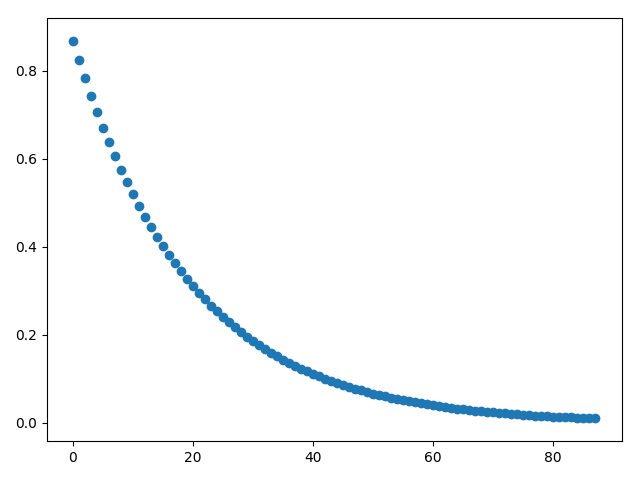
\includegraphics[scale=.35]{q1.png}
\end{figure}
The value iteration find the same policy $\pi^*$ and:
$$ v^* = [15.204, 16.361, 17.819] $$
\subsection{Question 3}
The exact policy iteration returned the same policy.\\
To compare both algorithm we used the $timeit$ module of python.\\
\begin{tabular}{|c|c|}
\hline 
 & Mean of 100 runs \\ 
\hline 
VI & 0.00208620 \\ 
\hline 
PI & 0.00179925 \\ 
\hline 
\end{tabular} 
\newpage
\section{Reinforcement Learning}
\subsection{Question 4}
\begin{figure}[h]
\centering
\caption{$ J_n - J^{\pi} $}
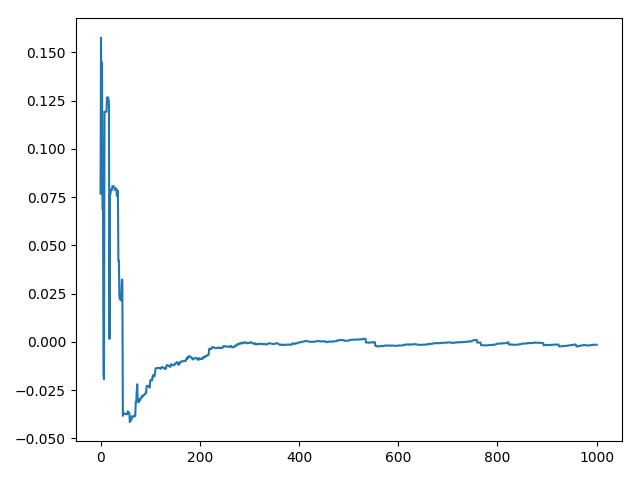
\includegraphics[scale=.35]{q4.png}
\end{figure}

\subsection{Question 5}
\begin{figure}[h]
\centering
\caption{$\parallel v^k - v^* \parallel_{\infty}$}
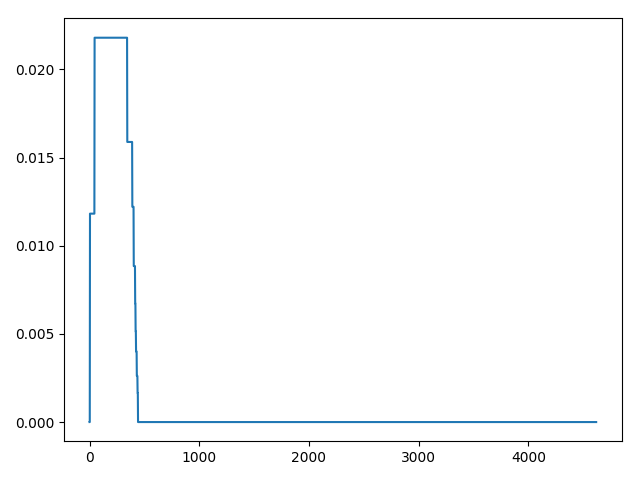
\includegraphics[scale=.35]{q5.png}
\end{figure}
\end{document}